\section{Appendix Section}
\label{sec:appendix_section}

\subsection{Additional SDFusion Fine-tuning results}
\label{sec:appendic_fine_tuning}

\iffalse
\begin{figure}[h]
  \centering
  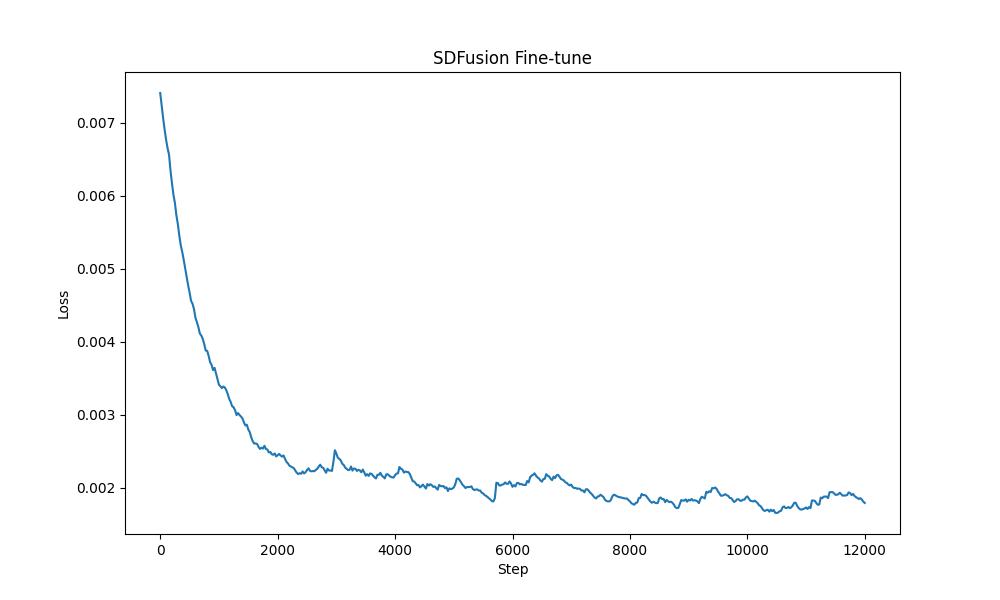
\includegraphics[width=\linewidth]{figs/sdfusion_finetune_loss_plot.png}
  \caption{Loss curve of our SDFusion fine-tune (smoothed).}
  \label{fig:finetune}
\end{figure}

\begin{figure}[h]
  \centering
  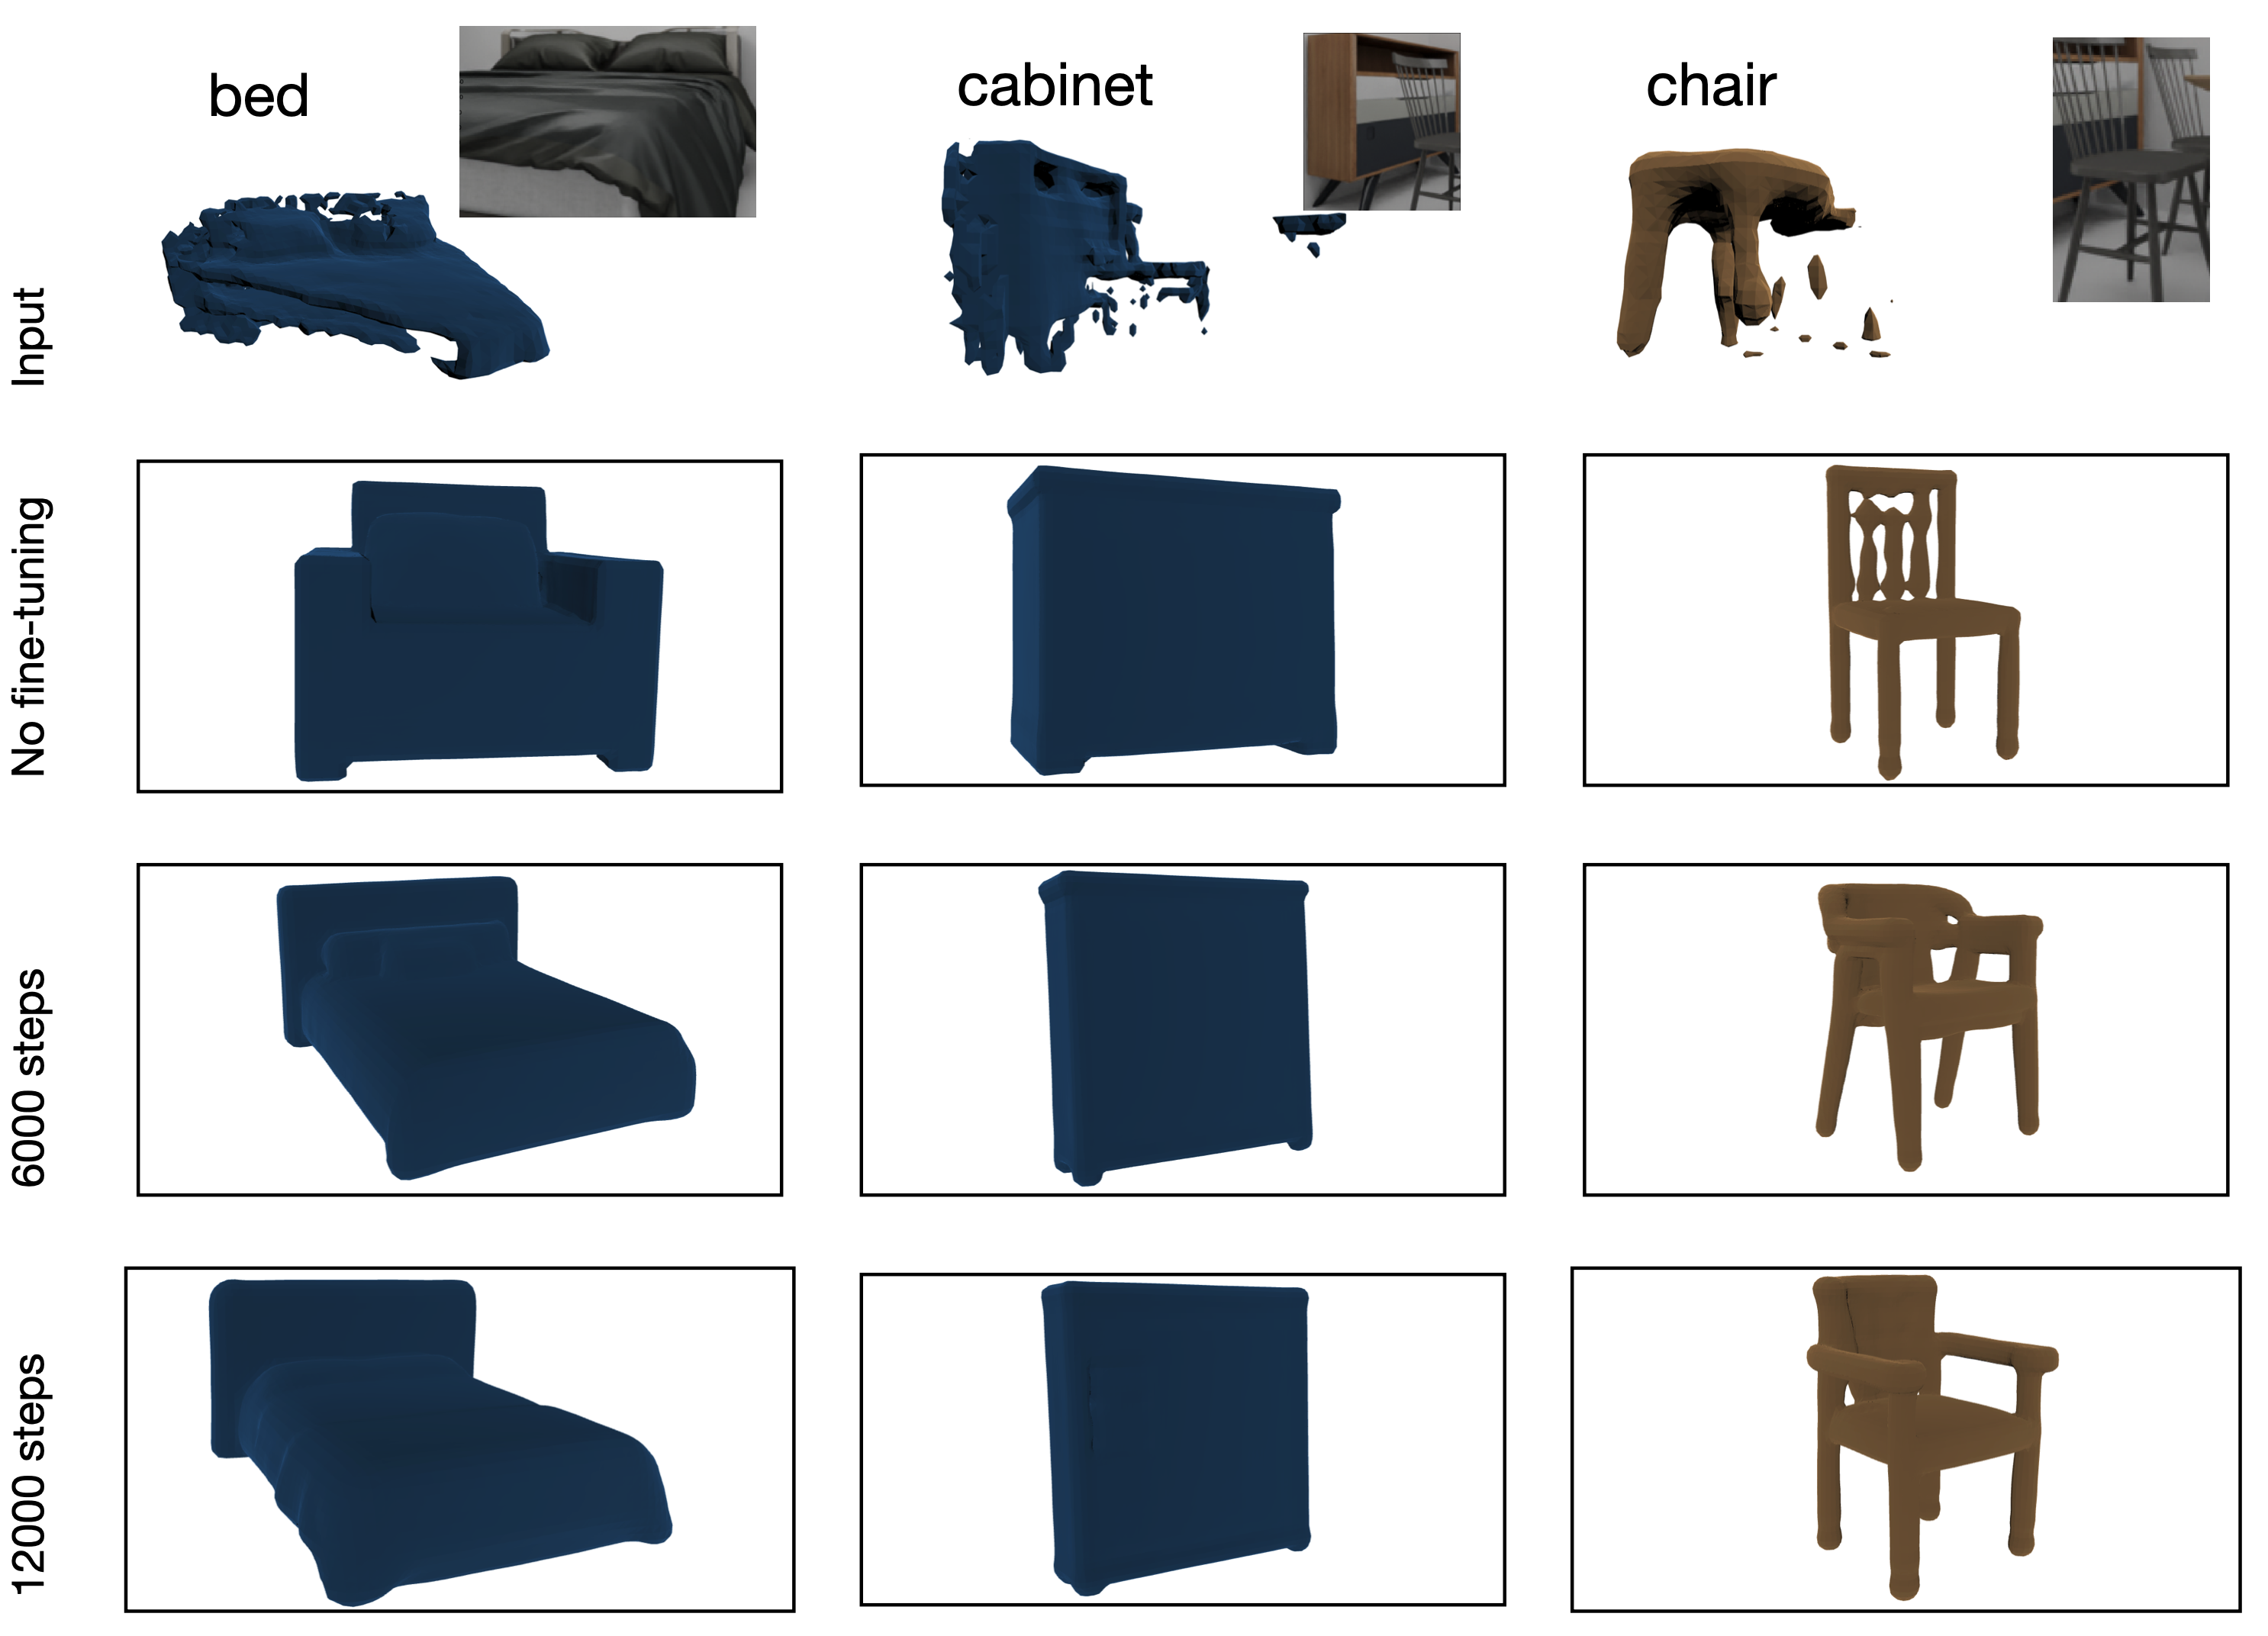
\includegraphics[width=80mm, scale=1]{images/image4.png}
  \caption{Fine-tuning results for SDFusion}
\end{figure}
\fi

\begin{figure*}
  \centering
  \begin{minipage}{0.49\linewidth}
    \centering
  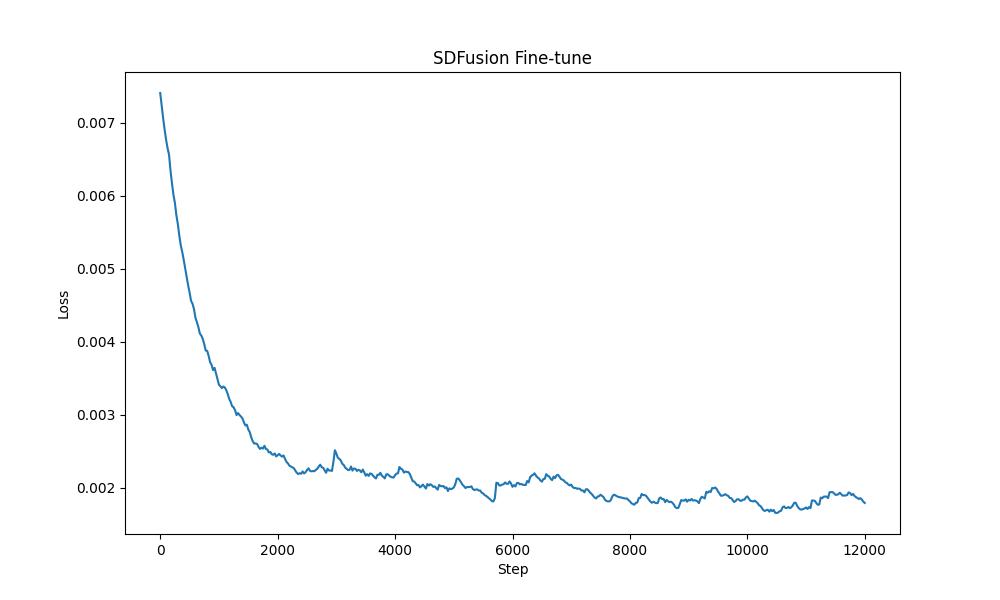
\includegraphics[width=\linewidth]{figs/sdfusion_finetune_loss_plot.png}
    \caption{Loss curve of our SDFusion fine-tune (smoothed).}
  \label{fig:finetune}
  \end{minipage}
  \hfill
  \begin{minipage}{0.49\linewidth}
    \centering
  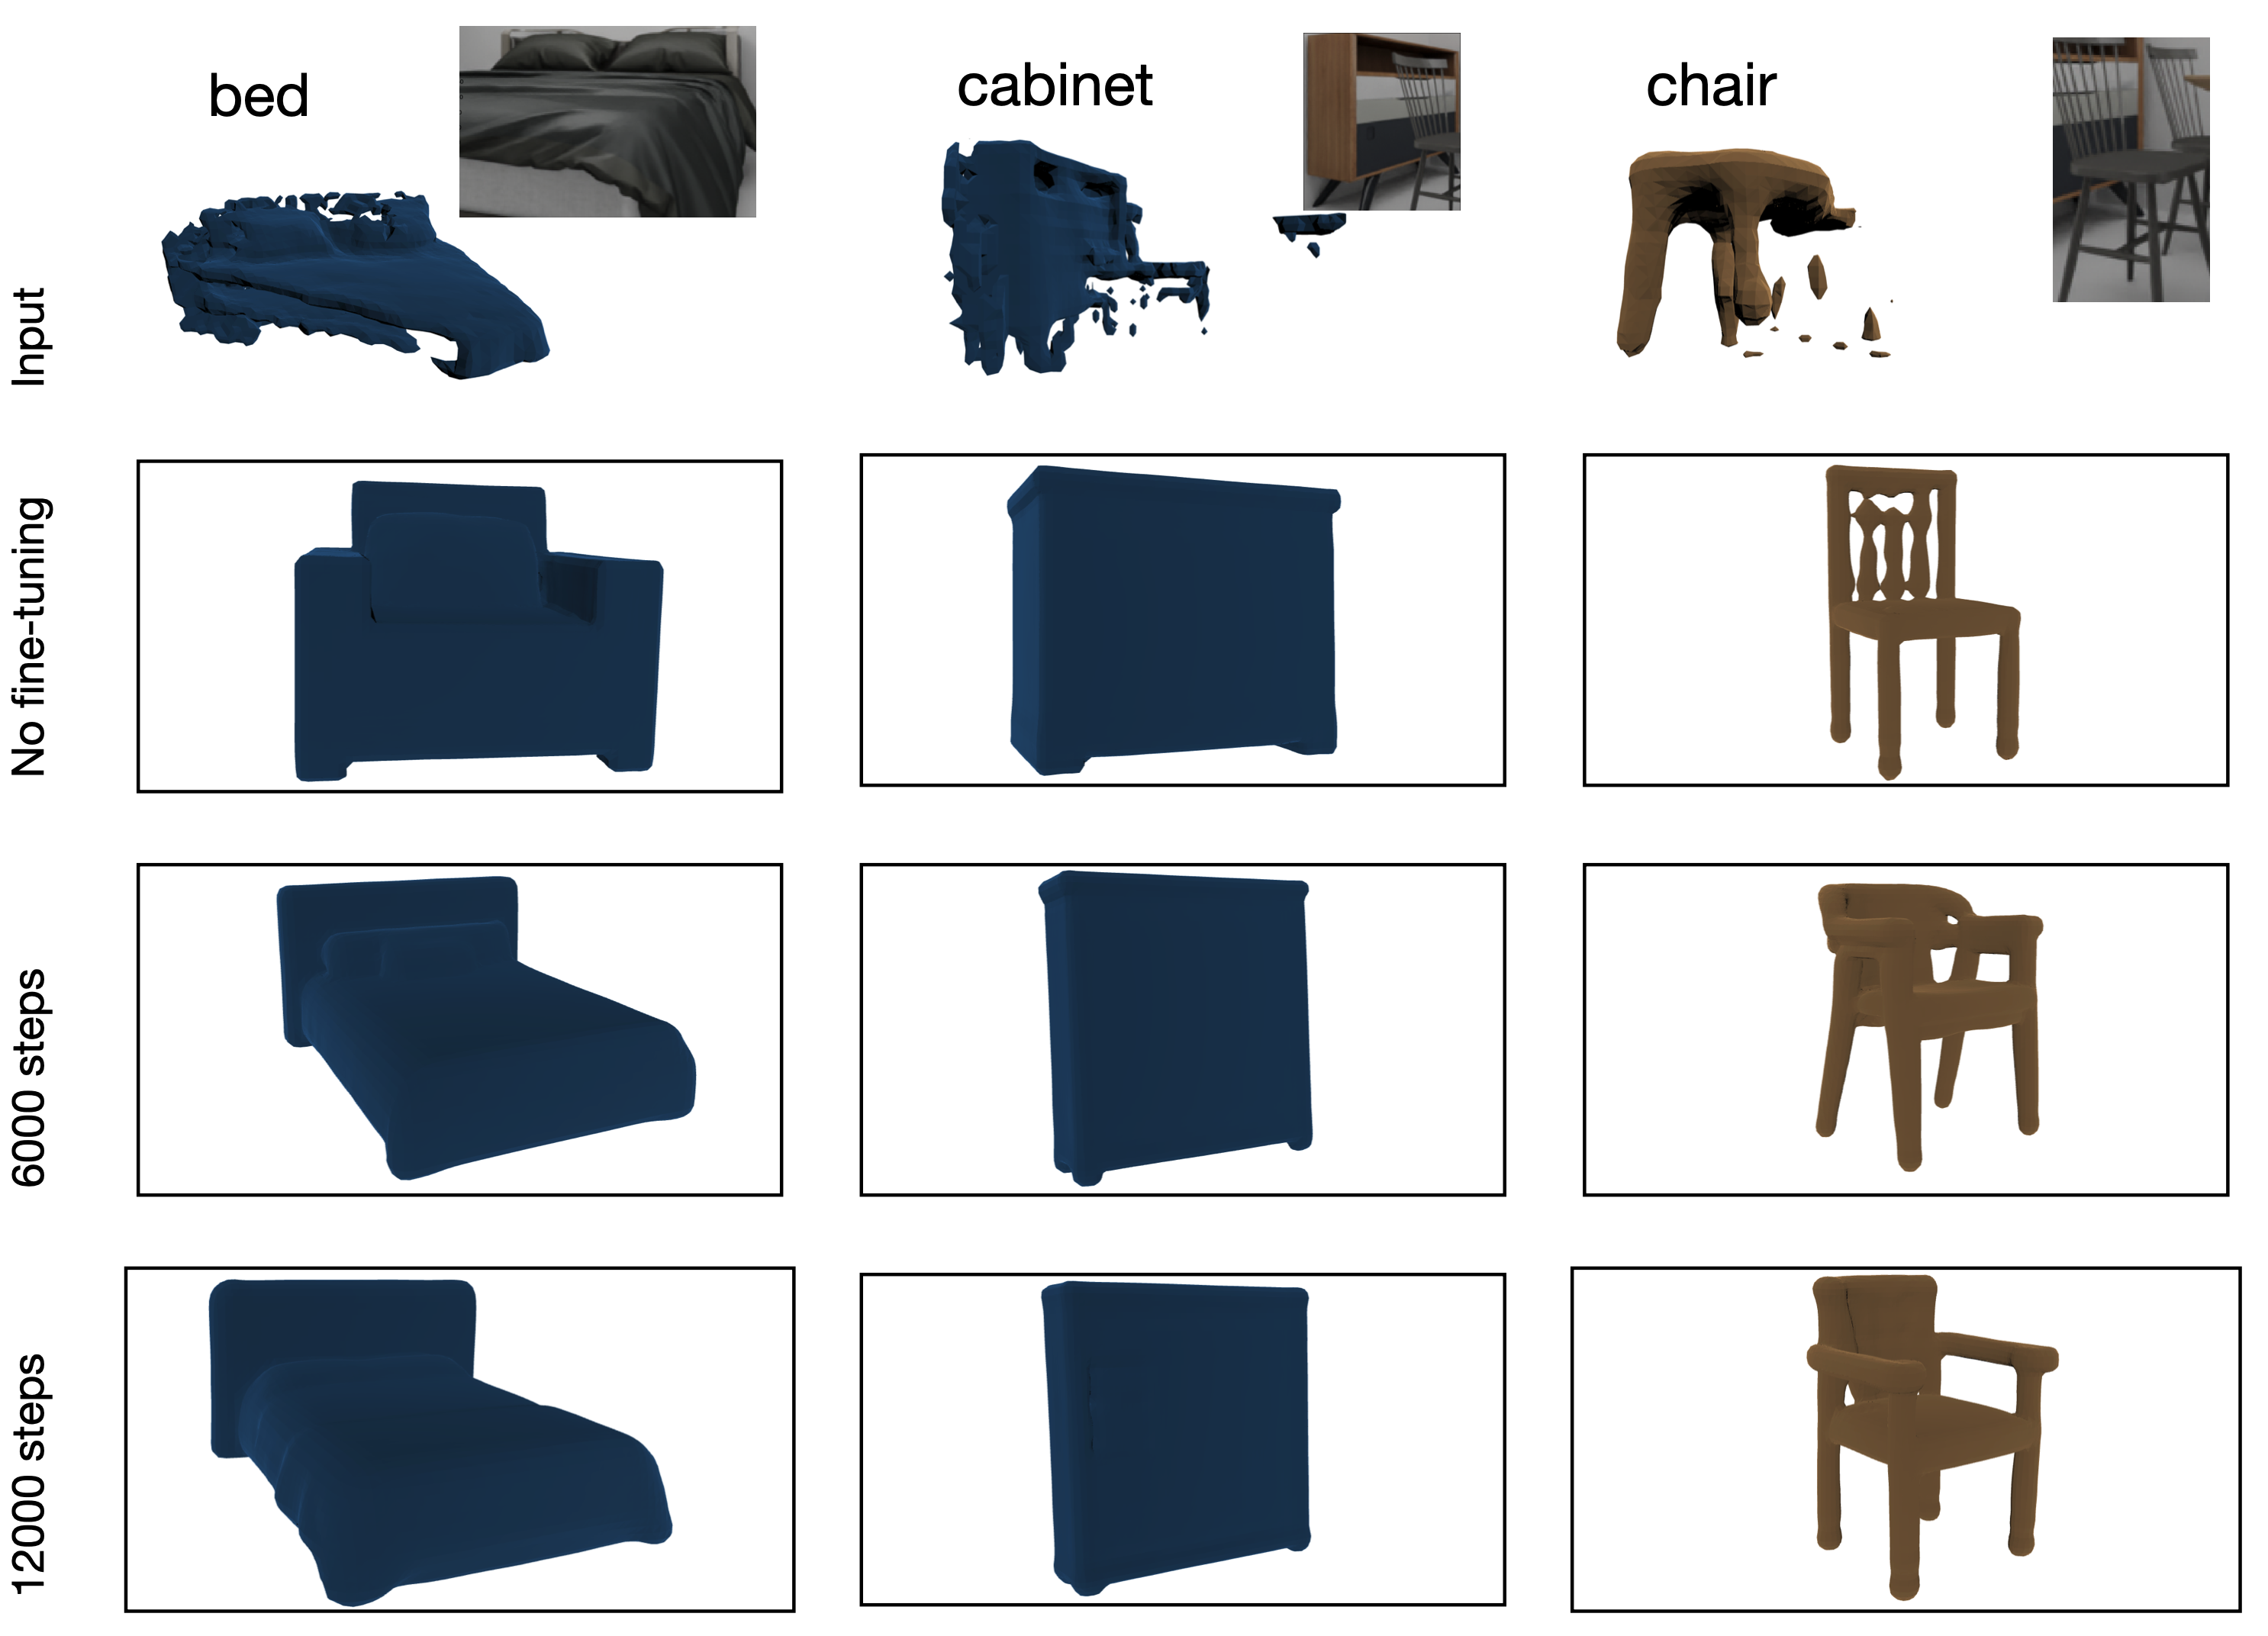
\includegraphics[width=\linewidth]{images/image4.png}
    \caption{Effect of fine-tuning SDFusion on reconstruction results. The process of fine-tuning significantly enhances our capacity to generate objects that more accurately align with those presented in Front3D. A notable improvement is observed in the refined geometries of beds. Prior to fine-tuning, the standard SDFusion model produced representations resembling armchairs; however, post-fine-tuning, the model successfully generates geometries that appropriately resemble beds.}
    \label{fig:short-b}
  \end{minipage}
\end{figure*}

\subsection{Additional Panoptic Model Training Results}

\begin{figure*}
  \centering
  \begin{minipage}{0.49\linewidth}
    \centering
  \begin{subfigure}[b]{0.45\linewidth}
    \centering
    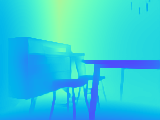
\includegraphics[width=\linewidth]{figs/depth_ours.png}
    \label{subfig:sub1}
   \vspace*{-3mm} % Adjust vertical spacing between the caption and the images
  \caption{Depth map (ours).}
  \end{subfigure}
  \hfill
  \begin{subfigure}[b]{0.45\linewidth}
    \centering
    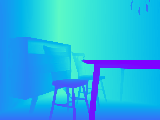
\includegraphics[width=\linewidth]{figs/depth_pan.png}
    \label{subfig:sub2}
   \vspace*{-3mm} % Adjust vertical spacing between the caption and the images
  \caption{Depth map (\citep{dahnert2021panoptic}).}
  \end{subfigure}

  \vspace{0.03\linewidth} % Adjust vertical spacing between rows of figures

  \begin{subfigure}[b]{0.45\linewidth}
    \centering
    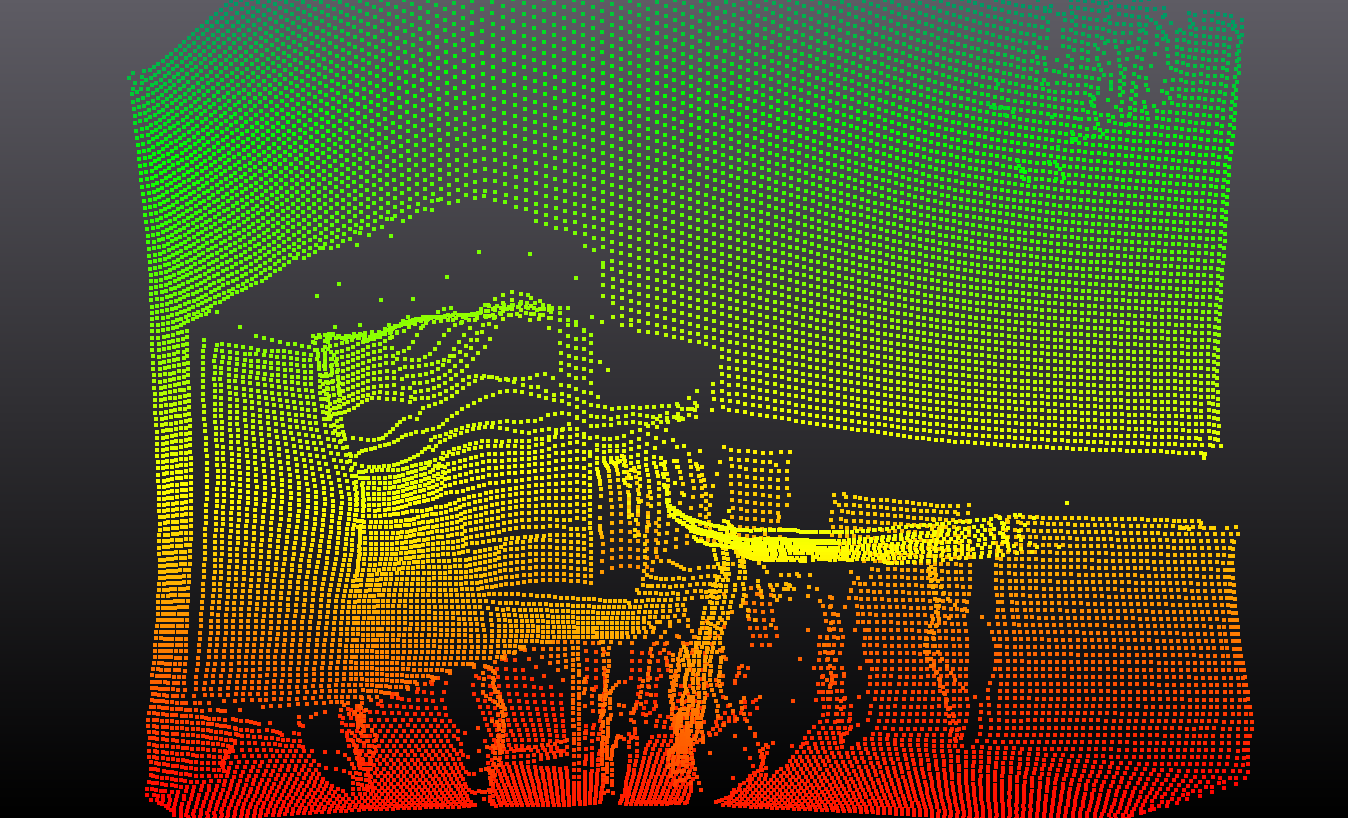
\includegraphics[width=\linewidth]{figs/depthply_ours.png}
    \label{subfig:sub3}
   \vspace*{-3mm} % Adjust vertical spacing between the caption and the images
   \caption{Geometry from depth (ours).}
  \end{subfigure}
  \hfill
  \begin{subfigure}[b]{0.45\linewidth}
    \centering
    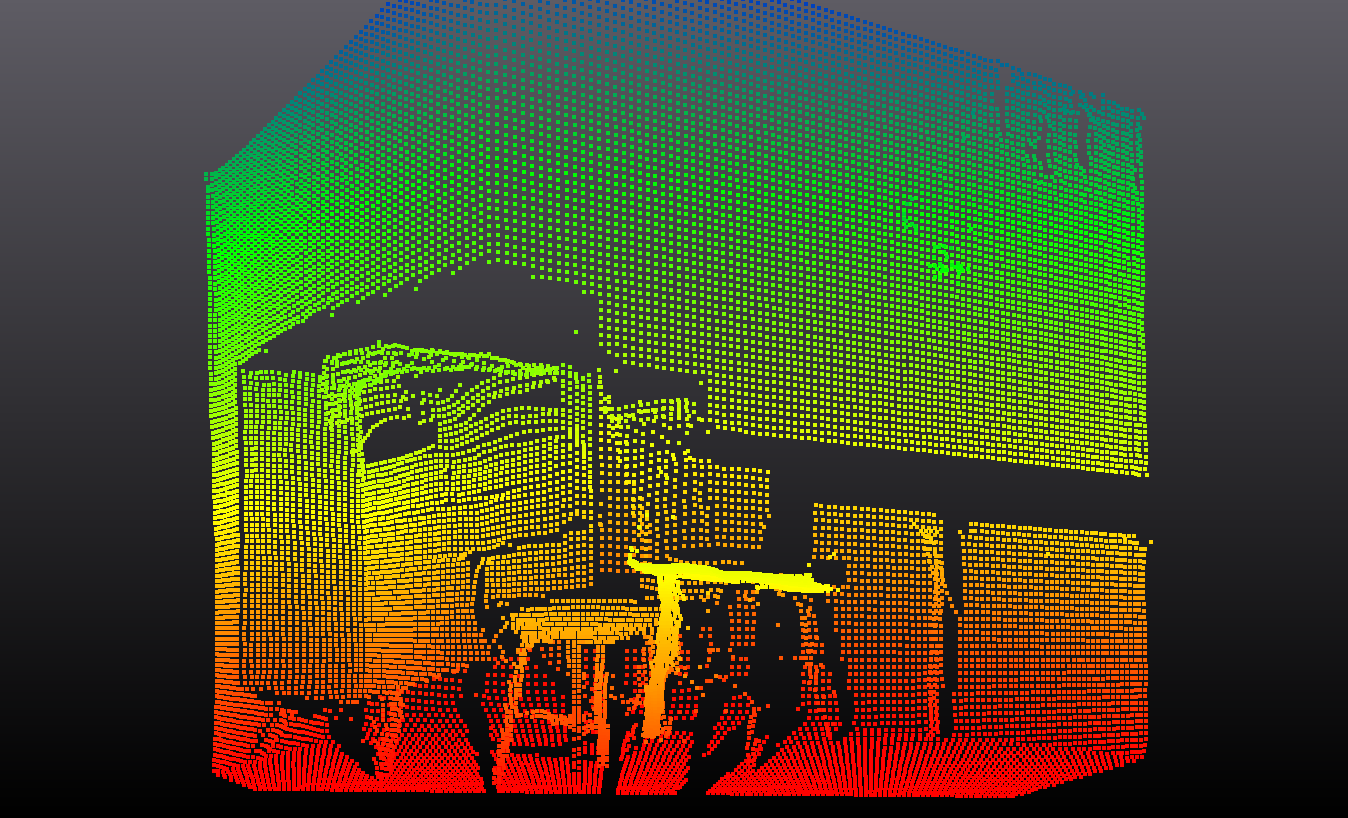
\includegraphics[width=\linewidth]{figs/depthply_pan.png}
    \label{subfig:sub4}
   \vspace*{-3mm} % Adjust vertical spacing between the caption and the images
   \caption{Geometry from depth (\citep{dahnert2021panoptic}).}
  \end{subfigure}

  \caption{2D results from the Panoptic 3D model. Our re-training results (left) vs. results from \citet{dahnert2021panoptic} (right).}
  \label{fig:qual_panoptic}
  \end{minipage}
  \hfill
  \begin{minipage}{0.49\linewidth}
    \centering
    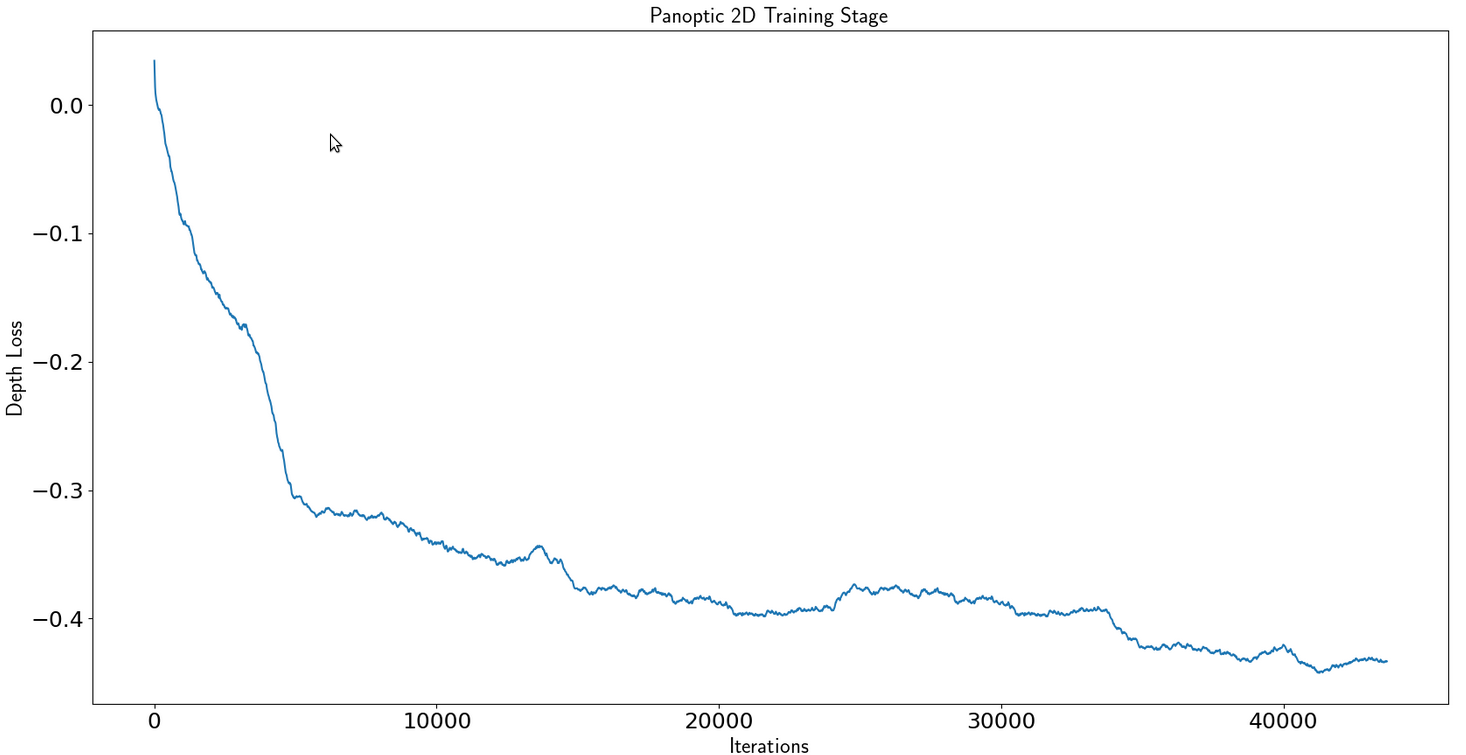
\includegraphics[width=\linewidth]{figs/depthloss.png}
    \caption{Depth loss curve for retraining of panoptic model (First 45k iterations).}
    \label{subfig:additional}
    \vspace*{-3mm} %
  \end{minipage}
\end{figure*}


\iffalse
\begin{figure}[h]
  \centering
  \begin{subfigure}[b]{0.45\linewidth}
    \centering
    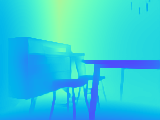
\includegraphics[width=\linewidth]{figs/depth_ours.png}
    \label{subfig:sub1}
   \vspace*{-3mm} % Adjust vertical spacing between the caption and the images
  \caption{Depth map (ours).}
  \end{subfigure}
  \hfill
  \begin{subfigure}[b]{0.45\linewidth}
    \centering
    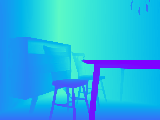
\includegraphics[width=\linewidth]{figs/depth_pan.png}
    \label{subfig:sub2}
   \vspace*{-3mm} % Adjust vertical spacing between the caption and the images
  \caption{Depth map (\citep{dahnert2021panoptic}).}
  \end{subfigure}

  \vspace{0.03\linewidth} % Adjust vertical spacing between rows of figures

  \begin{subfigure}[b]{0.45\linewidth}
    \centering
    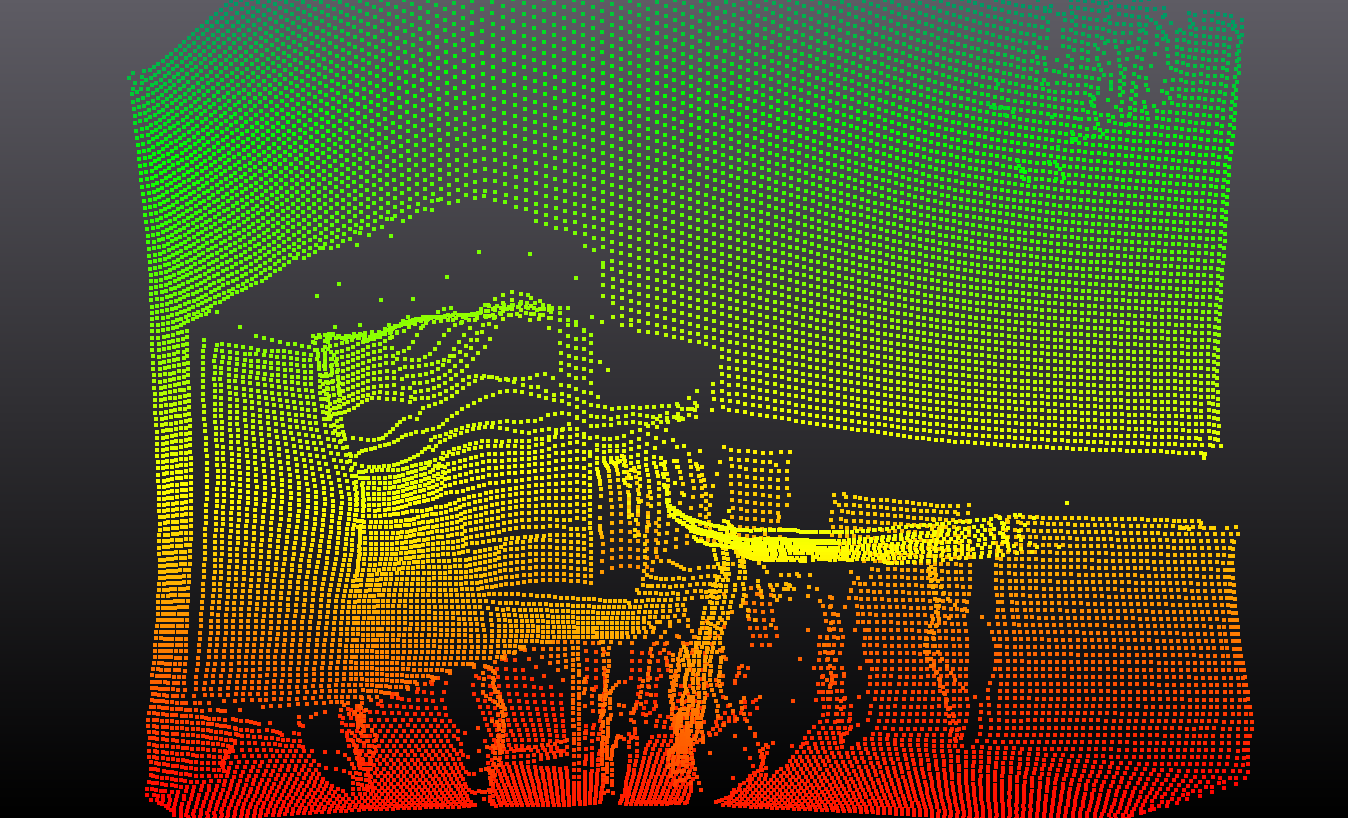
\includegraphics[width=\linewidth]{figs/depthply_ours.png}
    \label{subfig:sub3}
   \vspace*{-3mm} % Adjust vertical spacing between the caption and the images
   \caption{Geometry from depth (ours).}
  \end{subfigure}
  \hfill
  \begin{subfigure}[b]{0.45\linewidth}
    \centering
    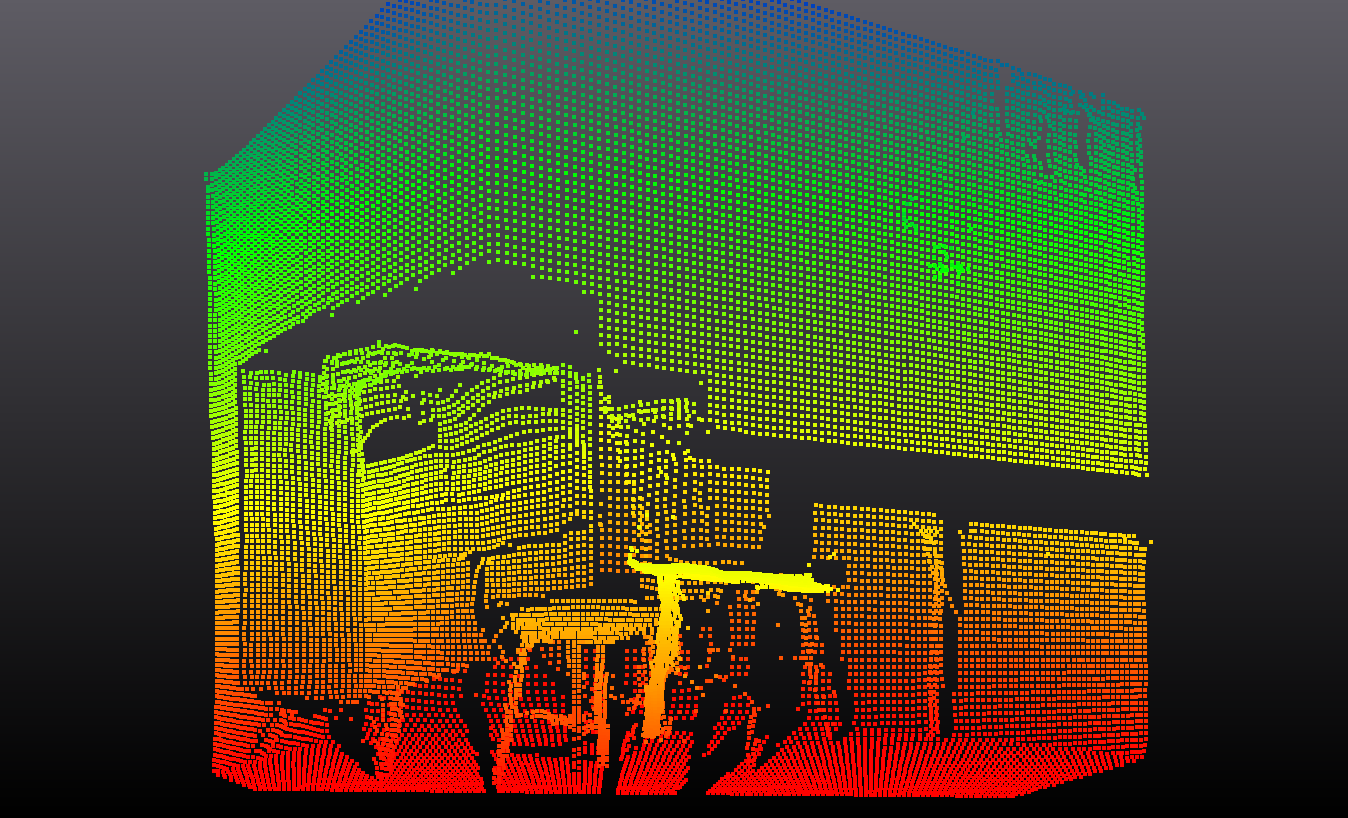
\includegraphics[width=\linewidth]{figs/depthply_pan.png}
    \label{subfig:sub4}
   \vspace*{-3mm} % Adjust vertical spacing between the caption and the images
   \caption{Geometry from depth (\citep{dahnert2021panoptic}).}
  \end{subfigure}

  \caption{2D results from the Panoptic 3D model. Our re-training results (left) vs. results from \citet{dahnert2021panoptic} (right).}
  \label{fig:qual_panoptic}
\end{figure}

\begin{figure*}[h]
  \centering
  \begin{subfigure}[b]{0.45\linewidth}
    \centering
    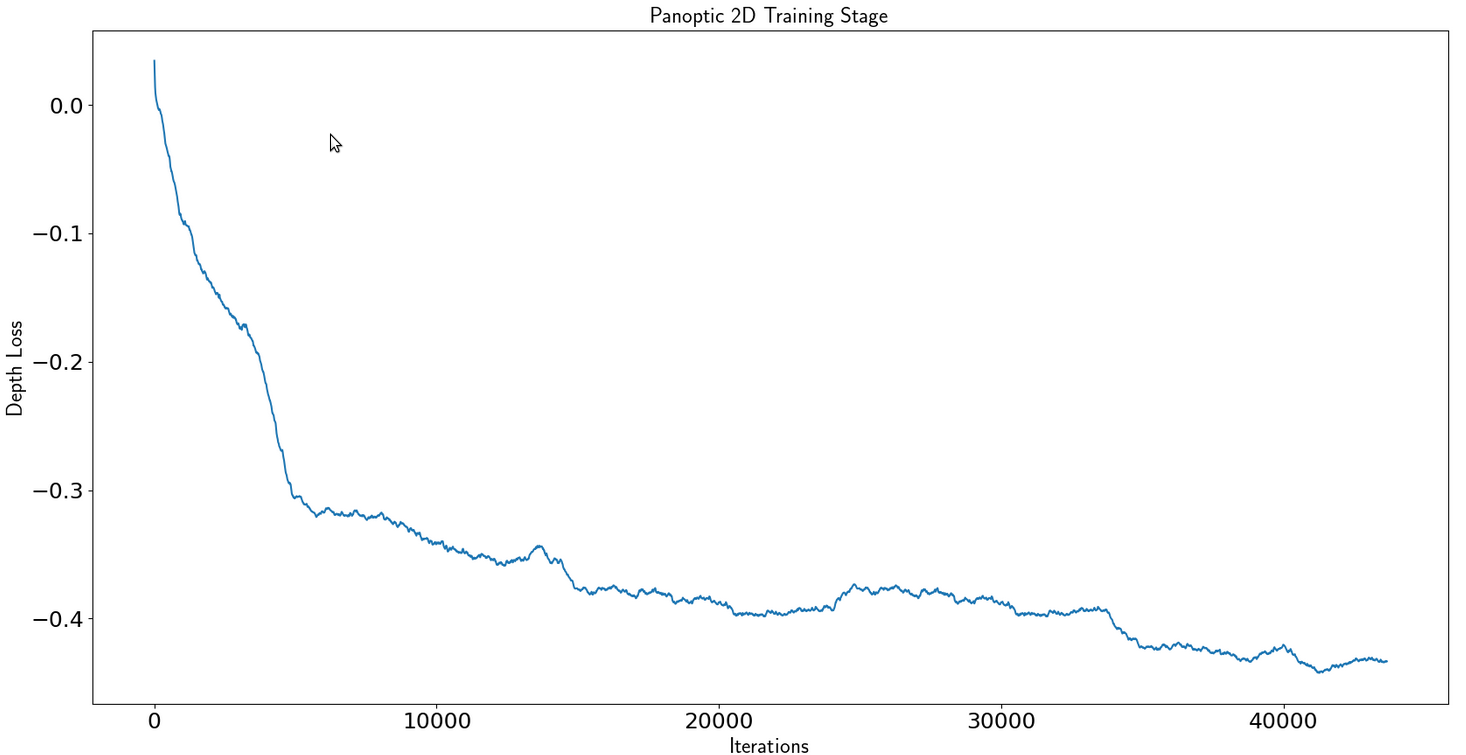
\includegraphics[width=\linewidth]{figs/depthloss.png}
    \caption{Depth loss curve for retraining of panoptic model (First 45k iterations).}
    \label{subfig:additional}
    \vspace*{-3mm} % Adjust vertical spacing between the caption and the image
  \end{subfigure}
\end{figure*}
\fi